\textbf{Pour les exercies \ref{TracerSymAxQuadri1} à \ref{TracerSymAxQuadri4} :} Tracer l'image de la figure suivante par la symétrie d'axe $(d)$.

\vspace{-2em}
\begin{minipage}[t]{0.45\textwidth}
    \exo{Représenter}{TracerSymAxQuadri1}
    
    \begin{figure}[H]
        \centering
        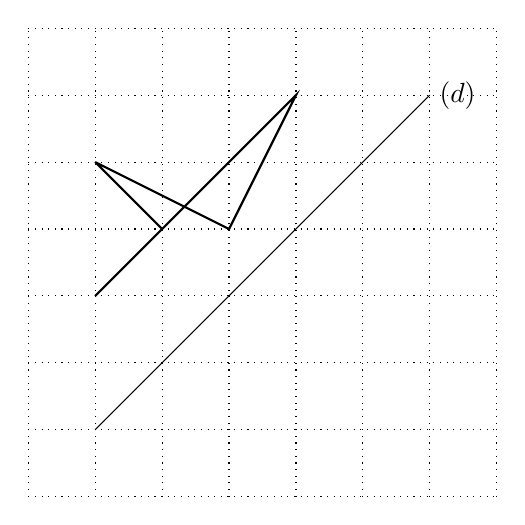
\begin{tikzpicture}[scale=0.85]
            \def\mypath{(-2,2) -- (-1,1) --(-2,0) -- (1,3)--(0,1)--(-2,2)}
            \draw [thick]\mypath ;
            \draw (-2,-2)--(3,3) node [right]{$(d)$} ;
            % \draw [cm={0,1,1,0,(0,0)}] \mypath;%Matrice de transformation inverse X et Y
            \draw [dotted](-3,-3) grid (4,4);
        \end{tikzpicture}
    \end{figure}
\end{minipage}
\hfill
\begin{minipage}[t]{0.45\textwidth}
    \exo{Représenter}{TracerSymAxQuadri2}
    
    \begin{figure}[H]
        \centering
        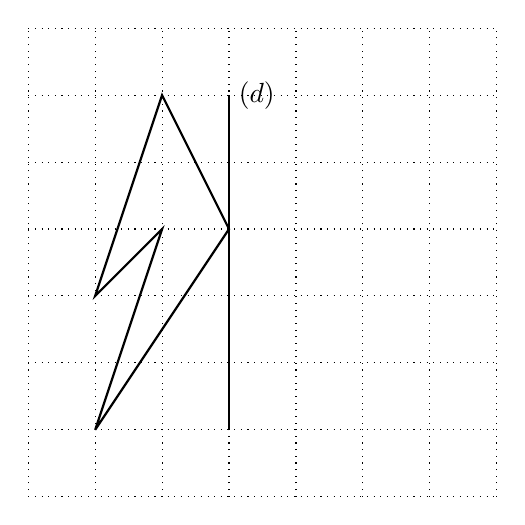
\begin{tikzpicture}[scale=0.85]
            \def\mypath{(-2,-2) -- (-1,1) --(-2,0) -- (-1,3)--(0,1)--(-2,-2)}
            \draw [thick]\mypath ;
            \draw (0,-2)--(0,3) node [right]{$(d)$} ;
            % \draw [cm={-1,0,0,1,(0,0)}] \mypath;%Matrice de transformation inverse X et Y
            \draw [dotted](-3,-3) grid (4,4);
        \end{tikzpicture}
    \end{figure}
\end{minipage}
\vspace{-1em}
\begin{minipage}[t]{0.45\textwidth}
    \exo{Représenter}{TracerSymAxQuadri3}
    
    \begin{figure}[H]
        \centering
        \begin{tikzpicture}[scale=0.85]
            \def\mypath{(-2,-2) -- (0,-1) --(3,-2) -- (2,0)--(-1,-1)--(-2,-2)}
            \draw [thick]\mypath ;
            \draw (-2,0)--(3,0) node [right]{$(d)$} ;
            % \draw [cm={1,0,0,-1,(0,0)}] \mypath;%Matrice de transformation inverse X et Y
            \draw [dotted](-3,-3) grid (4,4);
        \end{tikzpicture}
    \end{figure}
\end{minipage}
\hfill
\begin{minipage}[t]{0.45\textwidth}
    \exo{Représenter}{TracerSymAxQuadri4}
    
    \begin{figure}[H]
        \centering
        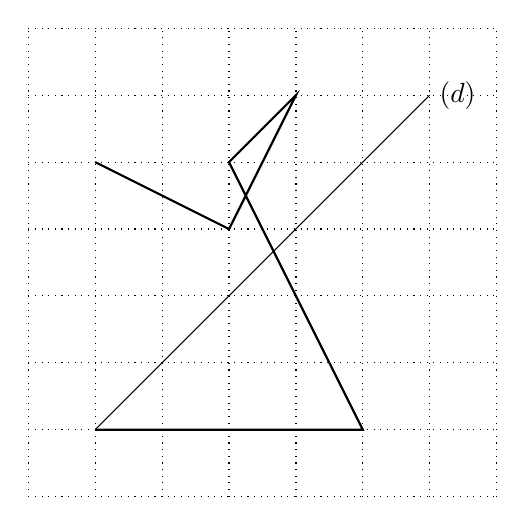
\begin{tikzpicture}[scale=0.85]
            \def\mypath{(-2,-2) -- (2,-2) --(0,2) -- (1,3)--(0,1)--(-2,2)}
            \draw [thick]\mypath ;
            \draw (-2,-2)--(3,3) node [right]{$(d)$} ;
            % \draw [cm={0,1,1,0,(0,0)}] \mypath;%Matrice de transformation inverse X et Y
            \draw [dotted](-3,-3) grid (4,4);
        \end{tikzpicture}
    \end{figure}
\end{minipage}

\vspace{2em}
\textbf{Pour les exercices \ref{TracerSymCentQuadri1} à \ref{TracerSymCentQuadri4} :} Tracer l'image de la figure suivante par la symétrie de centre $O$.
\vspace{-2em}

\begin{minipage}[t]{0.45\textwidth}
    \exo{Représenter}{TracerSymCentQuadri1}
    
    \begin{figure}[H]
        \centering
        \begin{tikzpicture}[scale=0.85]
            \tikzset{
                homothety at/.style args={#1 scaled by #2}{shift={($(#1)!#2!(0,0)$)},scale=#2},}
            \def\mypath{(-2,2) -- (-1,1) --(-2,0) -- (1,3)--(0,1)--(-2,2)}
            \draw [thick]\mypath ;
            \fill (0,0) coordinate (c) circle(2pt) node [above] {$O$};
            % \begin{scope}[homothety at=c scaled by -1]
            %     \draw \mypath;
            % \end{scope}
            \draw [dotted](-3,-3) grid (4,4);
        \end{tikzpicture}
    \end{figure}
\end{minipage}
\hfill
\begin{minipage}[t]{0.45\textwidth}
    \exo{Représenter}{TracerSymCentQuadri2}
    
    \begin{figure}[H]
        \centering
        \begin{tikzpicture}[scale=0.85]
            \tikzset{
                homothety at/.style args={#1 scaled by #2}{shift={($(#1)!#2!(0,0)$)},scale=#2},}
            \def\mypath{(-2,-2) -- (-1,1) --(-2,0) -- (-1,3)--(0,1)--(-2,-2)}
            \draw [thick]\mypath ;
            \fill (1,0) coordinate (c) circle(2pt) node [above] {$O$};
            % \begin{scope}[homothety at=c scaled by -1]
            %     \draw \mypath;
            % \end{scope}
            \draw [dotted](-3,-3) grid (4,4);
        \end{tikzpicture}
    \end{figure}
\end{minipage}

\begin{minipage}[t]{0.45\textwidth}
    \exo{Représenter}{TracerSymCentQuadri3}
    
    \begin{figure}[H]
        \centering
        \begin{tikzpicture}[scale=0.85]
            \tikzset{
                homothety at/.style args={#1 scaled by #2}{shift={($(#1)!#2!(0,0)$)},scale=#2},}
            \def\mypath{(-2,-2) -- (0,-1) --(3,-2) -- (2,0)--(-1,-1)--(-2,-2)}
            \draw [thick]\mypath ;
            \fill (0,0) coordinate (c) circle(2pt) node [above] {$O$};
            % \begin{scope}[homothety at=c scaled by -1]
            %     \draw \mypath;
            % \end{scope}
            \draw [dotted](-3,-3) grid (4,4);
        \end{tikzpicture}
    \end{figure}
\end{minipage}
\hfill
\begin{minipage}[t]{0.45\textwidth}
    \exo{Représenter}{TracerSymCentQuadri4}
    
    \begin{figure}[H]
        \centering
        \begin{tikzpicture}[scale=0.85]
            \tikzset{
                homothety at/.style args={#1 scaled by #2}{shift={($(#1)!#2!(0,0)$)},scale=#2},}
            \def\mypath{(-2,-2) -- (2,-2) --(0,2) -- (1,3)--(0,1)--(-2,2)}
            \draw [thick]\mypath ;
            \fill (0,1) coordinate (c) circle(2pt) node [above] {$O$};
            % \begin{scope}[homothety at=c scaled by -1]
            %     \draw \mypath;
            % \end{scope}
            \draw [dotted](-3,-3) grid (4,4);
        \end{tikzpicture}
    \end{figure}
\end{minipage}

\textbf{Pour l'exercice \ref{TracerTransQuadri1} à \ref{TracerTransQuadri4} :} Tracer l'image de la figure suivante par la translation qui envoie $A$ en $B$.
\vspace{-2em}

\begin{minipage}[t]{0.45\textwidth}
    \exo{Représenter}{TracerTransQuadri1}
    
    \begin{figure}[H]
        \centering
        \begin{tikzpicture}[scale=0.85]
            \def\mypath{(-2,2) -- (-1,1) --(-2,0) -- (1,3)--(0,1)--(-2,2)}
            \draw [thick]\mypath;
            % \draw [shift={(1,-3)}]\mypath ;
            \fill (2,3) coordinate (c) circle(2pt) node [above] {$A$};
            \fill (3,0) coordinate (c) circle(2pt) node [above] {$B$};
            \draw [dotted](-3,-3) grid (4,4);
        \end{tikzpicture}
    \end{figure}
\end{minipage}
\hfill
\begin{minipage}[t]{0.45\textwidth}
    \exo{Représenter}{TracerTransQuadri2}
    
    \begin{figure}[H]
        \centering
        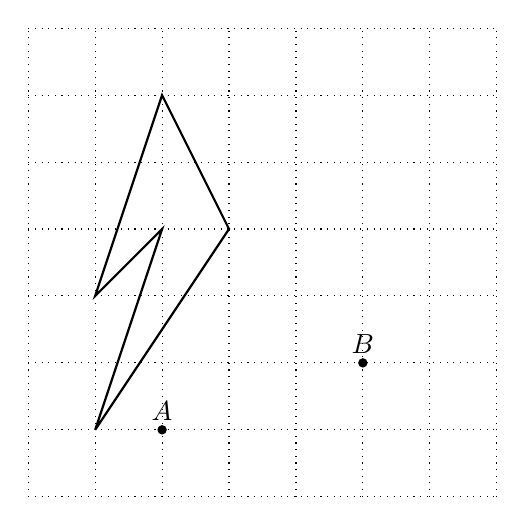
\begin{tikzpicture}[scale=0.85]
            \def\mypath{(-2,-2) -- (-1,1) --(-2,0) -- (-1,3)--(0,1)--(-2,-2)}
            \draw [thick]\mypath;
            % \draw [shift={(3,1)}]\mypath ;
            \fill (-1,-2) coordinate (c) circle(2pt) node [above] {$A$};
            \fill (2,-1) coordinate (c) circle(2pt) node [above] {$B$};
            \draw [dotted](-3,-3) grid (4,4);
        \end{tikzpicture}
    \end{figure}
\end{minipage}

\begin{minipage}[t]{0.45\textwidth}
    \exo{Représenter}{TracerTransQuadri3}
    
    \begin{figure}[H]
        \centering
        \begin{tikzpicture}[scale=0.85]
            \def\mypath{(-2,-2) -- (0,-1) --(3,-2) -- (2,0)--(-1,-1)--(-2,-2)}
            \draw [thick]\mypath;
            % \draw [shift={(1,3)}]\mypath ;
            \fill (-1,0) coordinate (c) circle(2pt) node [above] {$A$};
            \fill (0,3) coordinate (c) circle(2pt) node [above] {$B$};
            \draw [dotted](-3,-3) grid (4,4);
        \end{tikzpicture}
    \end{figure}
\end{minipage}
\hfill
\begin{minipage}[t]{0.45\textwidth}
    \exo{Représenter}{TracerTransQuadri4}
    
    \begin{figure}[H]
        \centering
        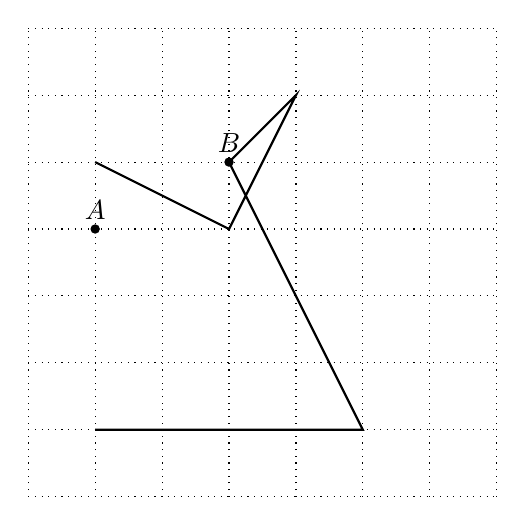
\begin{tikzpicture}[scale=0.85]
            \def\mypath{(-2,-2) -- (2,-2) --(0,2) -- (1,3)--(0,1)--(-2,2)}
            \draw [thick]\mypath;
            % \draw [shift={(2,1)}]\mypath ;
            \fill (-2,1) coordinate (c) circle(2pt) node [above] {$A$};
            \fill (0,2) coordinate (c) circle(2pt) node [above] {$B$};
            \draw [dotted](-3,-3) grid (4,4);
        \end{tikzpicture}
    \end{figure}
\end{minipage}
\newpage

\textbf{Pour les exercices \ref{TracerRotaQuadri1} à \ref{TracerRotaQuadri4} :} Tracer l'image par la rotation de centre $0$ avec l'angle donné.
\vspace{-2em}

\begin{minipage}[t]{0.45\textwidth}
    \exo{Représenter}{TracerRotaQuadri1}
    
    Angle $90$° dans le sens horairere.
    
    \begin{figure}[H]
        \centering
        \begin{tikzpicture}[scale=0.85]
            \def\mypath{(-2,2) -- (-1,1) --(-2,0) -- (1,3)--(0,1)--(-2,2)}
            \draw [thick]\mypath ;
            \fill (0,0) coordinate (c) circle(2pt) node [above] {$0$};
            % \draw [rotate=-90] \mypath ;
            \draw [dotted](-3,-3) grid (4,4);
        \end{tikzpicture}
    \end{figure}
\end{minipage}
\hfill
\begin{minipage}[t]{0.45\textwidth}
    \exo{Représenter}{TracerRotaQuadri2}
    
    Angle $90$° dans le sens anti-horairere.
    
    \begin{figure}[H]
        \centering
        \begin{tikzpicture}[scale=0.85]
            \def\mypath{(-2,-2) -- (-1,1) --(-2,0) -- (-1,3)--(0,1)--(-2,-2)}
            \draw [thick]\mypath ;
            \fill (0,0) coordinate (c) circle(2pt) node [above] {$0$};
            % \draw [rotate=90] \mypath ;
            \draw [dotted](-3,-3) grid (4,4);
        \end{tikzpicture}
    \end{figure}
\end{minipage}
\vspace*{-0.5em}
\begin{minipage}[t]{0.45\textwidth}
    \exo{Représenter}{TracerRotaQuadri3}
    
    Angle $90$° dans le sens horairere.
    
    \begin{figure}[H]
        \centering
        \begin{tikzpicture}[scale=0.85]
            \def\mypath{(-2,-2) -- (0,-1) --(3,-2) -- (2,0)--(-1,-1)--(-2,-2)}
            \draw [thick]\mypath ;
            \fill (0,0) coordinate (c) circle(2pt) node [above] {$0$};
            % \draw [rotate=-90] \mypath ;
            \draw [dotted](-3,-3) grid (4,4);
        \end{tikzpicture}
    \end{figure}
\end{minipage}
\hfill
\begin{minipage}[t]{0.45\textwidth}
    \exo{Représenter}{TracerRotaQuadri4}
    
    Angle $90$° dans le sens anti-horairere.
    
    \begin{figure}[H]
        \centering
        \begin{tikzpicture}[scale=0.85]
            \def\mypath{(-2,-2) -- (2,-2) --(0,2) -- (1,3)--(0,1)--(-2,2)}
            \draw [thick]\mypath ;
            \fill (0,0) coordinate (c) circle(2pt) node [above] {$0$};
            % \draw [rotate=90] \mypath ;
            \draw [dotted](-3,-3) grid (4,4);
        \end{tikzpicture}
    \end{figure}
\end{minipage}

\textbf{Pour les exercices \ref{TracerHomotQuadri1} à \ref{TracerHomotQuadri4} : }Tracer l'image par l'homothétie de centre $O$ avec le rapport donné.
\vspace{-2em}

\begin{minipage}[t]{0.45\textwidth}
    \exo{Représenter}{TracerHomotQuadri1}
    
    Rapport 2.
    
    \begin{figure}[H]
        \centering
        \begin{tikzpicture}[scale=0.85]
            \tikzset{
                homothety at/.style args={#1 scaled by #2}{shift={($(#1)!#2!(0,0)$)},scale=#2},}
            \def\mypath{(-2,2) -- (-1,1) --(-2,0) -- (1,3)--(0,1)--(-2,2)}
            \draw [thick]\mypath ;
            \fill (-1,2) coordinate (c) circle(2pt) node [above] {$O$};
            % \begin{scope}[homothety at=c scaled by 2]
            %     \draw \mypath;
            % \end{scope}
            \draw [dotted](-3,-3) grid (5,5);
        \end{tikzpicture}
    \end{figure}
\end{minipage}
\hfill
\begin{minipage}[t]{0.45\textwidth}
    \exo{Représenter}{TracerHomotQuadri2}
    
    Rapport 1,5.
    
    \begin{figure}[H]
        \centering
        \begin{tikzpicture}[scale=0.85]
            \tikzset{
                homothety at/.style args={#1 scaled by #2}{shift={($(#1)!#2!(0,0)$)},scale=#2},}
            \def\mypath{(-2,-2) -- (-1,1) --(-2,0) -- (-1,3)--(0,1)--(-2,-2)}
            \draw [thick]\mypath ;
            \fill (0,0) coordinate (c) circle(2pt) node [above] {$O$};
            % \begin{scope}[homothety at=c scaled by 1.5]
            %     \draw \mypath;
            % \end{scope}
            \draw [dotted](-3,-3) grid (5,5);
        \end{tikzpicture}
    \end{figure}
\end{minipage}

\begin{minipage}[t]{0.45\textwidth}
    \exo{Représenter}{TracerHomotQuadri3}
    
    Rapport -2.
    
    \begin{figure}[H]
        \centering
        \begin{tikzpicture}[scale=0.85]
            \tikzset{
                homothety at/.style args={#1 scaled by #2}{shift={($(#1)!#2!(0,0)$)},scale=#2},}
            \def\mypath{(-1,-2) -- (0,-1) --(3,-2) -- (2,0)--(-1,-1)--(-1,-2)}
            \draw [thick]\mypath ;
            \fill (1,-1) coordinate (c) circle(2pt) node [above] {$O$};
            % \begin{scope}[homothety at=c scaled by -2]
            %     \draw \mypath;
            % \end{scope}
            \draw [dotted](-3,-3) grid (5,5);
        \end{tikzpicture}
    \end{figure}
\end{minipage}
\hfill
\begin{minipage}[t]{0.45\textwidth}
    \exo{Représenter}{TracerHomotQuadri4}
    
    Rapport 2.
    
    \begin{figure}[H]
        \centering
        \begin{tikzpicture}[scale=0.85]
            \tikzset{
                homothety at/.style args={#1 scaled by #2}{shift={($(#1)!#2!(0,0)$)},scale=#2},}
            \def\mypath{(-2,-2) -- (2,-2) --(0,2) -- (1,3)--(0,1)--(-2,2)}
            \draw [thick]\mypath ;
            \fill (2,1) coordinate (c) circle(2pt) node [above] {$O$};
            % \begin{scope}[homothety at=c scaled by -0.5]
            %     \draw \mypath;
            % \end{scope}
            \draw [dotted](-3,-3) grid (5,5);
        \end{tikzpicture}
    \end{figure}
\end{minipage}